\documentclass[a4paper,12pt, notitlepage]{article}

\usepackage[top=25mm,bottom=25mm,left=25mm,right=25mm]{geometry}
%\usepackage{amsmath} 
\usepackage{graphicx}
%\usepackage{epstopdf}
\usepackage{listings}
\usepackage{color}
\usepackage{url}
\usepackage{setspace} 
%\usepackage[square, numbers]{natbib}
\usepackage{titlesec}
\usepackage{fancyhdr}
\usepackage[ddmmyyyy]{datetime}

\setstretch{1.44}
\setlength{\columnsep}{6mm}
\titleformat{\section}{\bfseries\large\scshape\filright}{\thesection}{1em}{}
\titleformat{\subsection}{\bfseries\normalsize\scshape\filright}{\thesubsection}{1em}{}


\renewcommand{\abstractname}{}
\newcommand{\captionfonts}{\footnotesize}
\renewcommand\thesection{\arabic{section}.}
\renewcommand\thesubsection{\arabic{section}.\arabic{subsection}}

\makeatletter
\long\def\@makecaption#1#2{
  \vskip\abovecaptionskip
  \sbox\@tempboxa{{\captionfonts #1: #2}}
  \ifdim \wd\@tempboxa >\hsize
    {\captionfonts #1: #2\par}
  \else
    \hbox to\hsize{\hfil\box\@tempboxa\hfil}
  \fi
  \vskip\belowcaptionskip}
    
\makeatother

\definecolor{dkgreen}{rgb}{0,0.6,0}
\definecolor{gray}{rgb}{0.5,0.5,0.5}
\definecolor{mauve}{rgb}{0.58,0,0.82}

\lstset{frame=tb,
	language=python,
	aboveskip=3mm,
	belowskip=3mm,
	showstringspaces=false,
	columns=flexible,
	basicstyle={\small\ttfamily},
	numbers=none,
	numberstyle=\tiny\color{gray},
	keywordstyle=\color{blue},
	commentstyle=\color{dkgreen},
	stringstyle=\color{mauve},
	breaklines=true,
	breakatwhitespace=true,
	tabsize=3
}

\pagestyle{fancy}
\fancyhf{}
\rhead{Getting Started: Adjustable Power}
\lhead{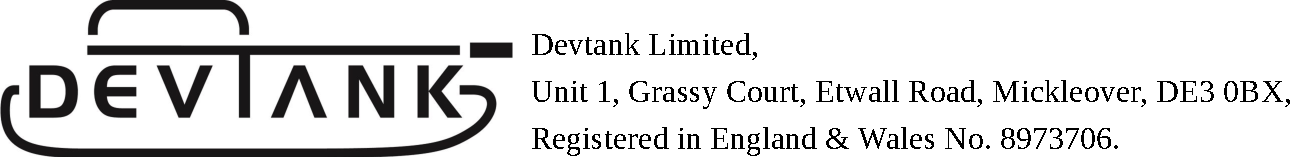
\includegraphics[height=1cm]{./Images/logo.pdf}}
\rfoot{Page \thepage}
\lfoot{}

\renewcommand{\dateseparator}{.}

\begin{document}
%%%%%%%%%%%%%%%%%%%%%%%%%%%%%%%%%%%%%%%%%%%%%%%%%%%%%%%%%%%%%%%%%%%%%%%%%%%%%%%%%%%%
\title{\textbf{\large{Getting Started: Adjustable Power}}}

\author{\normalsize{Devtank Ltd.} \\
        \small\textit{
        Harry Geyer}}
\date{\today}

\maketitle 
\thispagestyle{fancy}

%%%%%%%%%%%%%%%%%%%%%%%%%%%%%%%%%%%%%%%%%%%%%%%%%%%%%%%%%%%%%%%%%%%%%%%%%%%%%%%%%%%%

\begin{abstract} 
\noindent
This document is a guide for using the adjustable power supply on Devtank's HILTOP.
\end{abstract}
\vspace{11mm}

\newpage
\tableofcontents
\newpage

%%%%%%%%%%%%%%%%%%%%%%%%%%%%%%%%%%%%%%%%%%%%%%%%%%%%%%%%%%%%%%%%%%%%%%%%%%%%%%%%%%%%
\section{Prerequisites}
\label{sec: prereq}

\textbf{Hardware:}

\begin{enumerate}
  \item HILTOP
  \item Multimeter
  \item Linux machine to work with (Suggested)
\end{enumerate}

\noindent
\textbf{Software:}

\begin{enumerate}
  \item HILTOP development image
  \item libdevtankreborn library
\end{enumerate}

%%%%%%%%%%%%%%%%%%%%%%%%%%%%%%%%%%%%%%%%%%%%%%%%%%%%%%%%%%%%%%%%%%%%%%%%%%%%%%%%%%%%
\newpage
\section{Power Controller}
\label{sec: Pwrctl}

\subsection{Normal Use}
\label{ssec: normalPwrctl}

The adjustable power supply class is called \lstinline!power_controller_t! located in \url{./dtlib/pylibapps/dt_db_base.py}.

\begin{lstlisting}[label={lst: normalUse}, caption={A normal way of using the power controller object.}]
import dt_db_base
pwr_ctl = dt_db_base.power_controller_t()
pwr_ctl.load("./libhw/config_example.yaml")
pwr_ctl.power_supply_enabled = True
pwr_ctl.set_voltage_and_wait(5)
pwr_ctl.power_out_enabled = True
\end{lstlisting}

Listing \ref{lst: normalUse} shows that the adjustable power control per test scripts are simple to setup and use. In this script it will set to 5V and wait 3 seconds (default). An additional parameter can be entered into the \lstinline!set_voltage_and_wait! to set a different wait time. 

The loaded yaml file is the power control config file, an example can be found \url{./libhw/config_example.yaml}. This contains the scales and offset to convert the ADC measured by the HILTOP to the DC voltage required. It is recommended that a multimeter is used to measure at various voltages to ensure a good scale and offset (will vary depending on hardware). 

Once the object has been created, used and turned off, it cannot be turned back on, a new object needs to be created (a restart of the test group is fine).

\subsection{Binding}
\label{ssec: bindingPwrctl}

For multiple scripts to use the power controller it will need to be added to the binding. The best place would be in \lstinline!bus! class inside the binding, found in \url{./apps/app/example_lib}. For scripts to be able to control the voltage, it needs to be exposed to the \lstinline!dev_t! class.

First step is to give link the bus and the power controller object together:

\begin{lstlisting}[label={lst: adjpwrStruct0},caption={Make an object for the power controller.}]
from dt_db_base import power_controller_t
class example_bus(object):
    def __init__(self):
        self._obj = None
        self.pwr_ctl = power_controller_t()
\end{lstlisting}

Now the power control object is an attribute of the bus, a way to enable and disable the power controller. 

\begin{lstlisting}[label={lst: adjpwrStruct1},caption={}]
    def _enable_pwr(self):
        self.has_pwr_control = False
        if not self.pwr_ctl.is_setup:
            self.has_pwr_control = self.pwr_ctl.load(b"./hiltop.yaml")
        else:
            self.has_pwr_control = True
    def _disable_pwr(self):
        if self.has_pwr_control and self.pwr_ctl.is_setup:
            self.pwr_ctl.power_out_enabled = False
            self.pwr_ctl.shutdown()
\end{lstlisting}

Adding these to \lstinline!open! and \lstinline!close! enable on start and disable on exit:

\begin{lstlisting}[label={lst: adjpwrStruct2},caption={Enabling power supply for the duration of the test groups.}]
    def open(self):
        self._enable_pwr()
        self._obj = example_bus_con()
        return self._obj
    def off(self):
        if not self.has_pwr_control or not self.pwr_ctl.is_setup:
            self.has_pwr_control = self.pwr_ctl.load(b"hiltop.yaml")
        self._disable_pwr()
    def close(self):
        if self.autooff:
            self.off()
        self._obj = None
\end{lstlisting}

Now there are a lot of new attributes that have been used for these functions, they will be required to be defined. To update \lstinline!__init__! to contain attributes used in controlling the power controller:

\begin{lstlisting}[label={lst: adjpwrStruct3},caption={Including new attributes.}]
    def __init__(self):
        self._obj = None
        self.pwr_ctl = power_controller_t()
        self.pwr_ctl.use_stderr = True
        self.has_pwr_control = False
        self.autooff = True
\end{lstlisting}

Now finally the framework for the adjustable power controller is ready. Check \url{./dtlib/pylibapps/dt_db_base.py} for availble functions. This is an example of how you may want to control the power:

\begin{lstlisting}[label={lst: adjpwrStruct4},caption={Function for setting power and waiting.}]
    def set_pwr(self, v):
        v_set = False
        if self.has_pwr_control:
            if not self.pwr_ctl.power_supply_enabled:
                self.pwr_ctl.power_supply_enabled = True
                self.pwr_ctl.set_voltage_and_wait(v)
                v_set = True
            self.pwr_ctl.power_out_enabled = True
        return v_set
\end{lstlisting}

There is a problem as it currently is in the \lstinline!bus! class and so unreachable by the test scripts. Making it reachable can be done two ways, hand the bus object to the dev object, or hand over a function for controlling power to the dev object.

This document will discuss the former as can be used more generically. This handing over can be done by adding \lstinline!self! as a parameter to the \lstinline!example_bus_con()! in the \lstinline!open! function. The \lstinline!example_bus_con! class must now be changed to allow for this. This would however create a cyclic dependancy so weakref should be used to avoid this.

\begin{lstlisting}[label={lst: adjpwrStruct5},caption={Handing the bus object forwards to the bus\_con}]
import weakref
class mb_prod_bus_con(object):
    def __init__(self, _bus_obj):
        self._devices = []
        self.bus_obj = weakref.ref(_bus_obj)
    def ready_devices(self, known_devices):
        if len(known_devices):
            self._devices = [ example_dev_t(known_devices[0].uuid) ]
        else:
            self._devices = []
\end{lstlisting}

Now the \lstinline!bus_con! has access to the power controller, but for the dev object to the same must be done for the \lstinline!bus_con! to \lstinline!dev!. Add \lstinline!self.bus_obj()! as a second parameter to \lstinline!example_dev_t! and then inside the \lstinline!dev! class declare the bus object (with weakref) locally.

\begin{lstlisting}[label={lst: adjpwrStruct6},caption={Final hand over to dev object.}]
class example_dev_t(object):
    def __init__(self, uuid, _bus_obj):
        self._uuid    = uuid
        self._bus_obj = weakref.ref(_bus_obj)
    @property
    def bus_obj(self):
        return self._bus_obj()
\end{lstlisting}

Now \lstinline!self.bus_obj! is the bus object, the function to control the power is accessible, just need to call it from dev:

\begin{lstlisting}[label={lst: adjpwrStruct6},caption={Setting the function in the dev class.}]
    def set_v(self, v, t=3):
        return example_bus.set_pwr(self.bus_obj, v, t)
\end{lstlisting}

Now in the test scripts \lstinline!dev.set_v(10)! can be used to set the output voltage to be 10V for 3 seconds. Recommend an accuracy check with a multimeter.

Alternatively, single functions or just the power object could be handed through to produce a less cluttered dev object. 

%%%%%%%%%%%%%%%%%%%%%%%%%%%%%%%%%%%%%%%%%%%%%%%%%%%%%%%%%%%%%%%%%%%%%%%%%%%%%%%%%%%%
\small{
\begin{thebibliography}{99}

\setlength{\itemsep}{-2mm}

\bibitem{Webpage} Page Title,
                  Author {\url{https://www.url.org/}} {Accessed: dd.mm.yy}.
\bibitem{Book} Author, 
                  {\em Book Name}. Publisher {\bf Edition}, Pages (Publish Year).

\end{thebibliography}
}

\end{document}